\documentclass{beamer}

\usepackage{subcaption}
\usepackage{float}

% For more themes, color themes and font themes, see:
% http://deic.uab.es/~iblanes/beamer_gallery/index_by_theme.html

\mode<presentation>
{
  \usetheme{Berkeley}      % or try Darmstadt, Madrid, Warsaw, ...
  \usecolortheme{whale} % or try albatross, beaver, crane, ...
  \usefonttheme{default}  % or try serif, structurebold, ...
  \setbeamertemplate{navigation symbols}{}
  \setbeamertemplate{caption}[numbered]
} 

\usepackage[english]{babel}
\usepackage[utf8]{inputenc}
\usepackage[T1]{fontenc}

\title[SC 635 Labwork]{SC635: Advanced Topics in Mobile Robotics\\Labwork Report}
\author{Aaron John  Sabu}
\institute{170070050\\ Department of Electrical Engineering\\ IIT Bombay}
\date{March 3, 2020}

\begin{document}

\maketitle

\section{A1}

\begin{frame}{Assignment 1}
  \centering
  \textbf{Assignment 01:\\Waypoint Generation and Trajectory Tracking\\ with \textit{turtlebot}}
\end{frame}


\subsection{Progress}
\begin{frame}{Progress}
\begin{itemize}
    \item The developed scripts for waypoint generation as well as trajectory tracking had been submitted as part of the entire workspace
    \item Due to issues on my laptop, I had used a friend's laptop. The successful debugging of the code was not possible at that point of time
\end{itemize}
\end{frame}

\section{A2}

\begin{frame}{Assignment 2}
  \centering
  \textbf{Assignment 02:\\Obstacle Avoidance with Range Sensing}
\end{frame}

\subsection{Progress}
\begin{frame}{Progress}
\begin{itemize}
    \item Tangent Bug has been completed successfully, working in both worlds.
    \item Bug 2 has been designed. However, the simulation is not working and several efforts to debug have turned out futile.
\end{itemize}
\end{frame}

\subsection{Tangent Bug}
\begin{frame}{Tangent Bug}
\begin{figure}[H]
    \centering
    \begin{subfigure}{\textwidth}
        \centering
        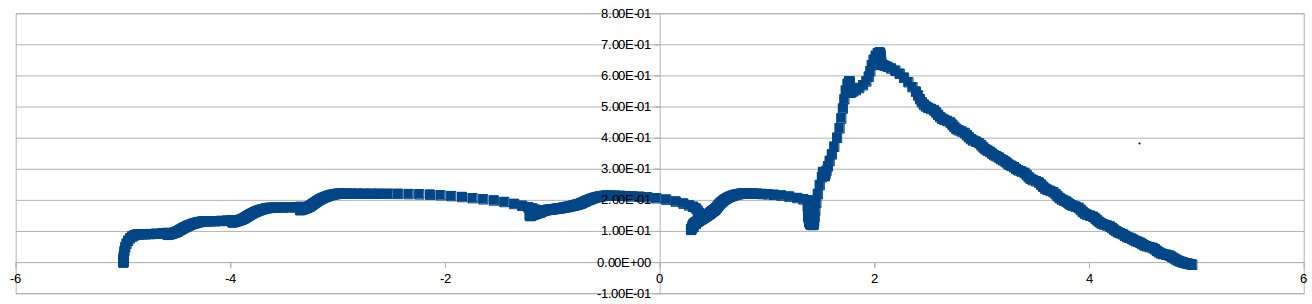
\includegraphics[width=\textwidth]{A2_TangBug_XY_1.png}
        \caption{World 1}
    \end{subfigure}
    \begin{subfigure}{\textwidth}
        \centering
        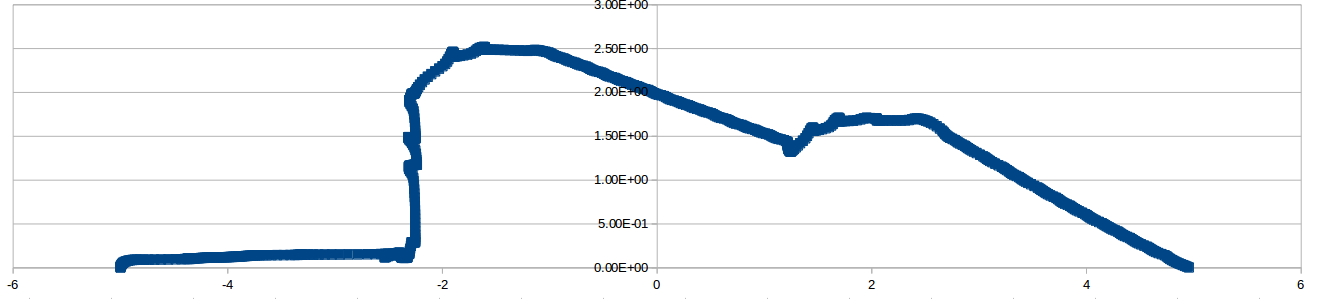
\includegraphics[width=\textwidth]{A2_TangBug_XY_2.png}
        \caption{World 2}
    \end{subfigure}
    \caption{X-Y Plot}
\end{figure}
\end{frame}

\subsection{Tuning Parameters}
\begin{frame}{Tuning Parameters}
\begin{itemize}
    \item The distance cutoff chosen was 0.3 m; i.e., when the robot was closer than 0.3 m to the destination, the iterator was incremented
    \item The proportionality constant for linear motion was 0.40 and that for angular motion was 0.15
    \item The maximum angular error permitted for high linear velocities was \(2^\circ\); i.e., at a heading with an angular error more than \(2^\circ\), the robot corrects the heading before moving forward significantly
\end{itemize}
\end{frame}

\section{A3}

\begin{frame}{Assignment 3}
  \centering
  \textbf{Assignment 03:\\Trilateration with Ground Mobile Robot}
\end{frame}

\subsection{Progress}
\begin{frame}{Progress}
\begin{itemize}
    \item The labwork has been successfully completed with variances up to (0.10, 0.10, 0.10).
\end{itemize}
\end{frame}

\subsection{Trajectory}
\begin{frame}{Trajectory}
\begin{figure}[H]
    \centering
    \begin{subfigure}{0.45\textwidth}
        \centering
        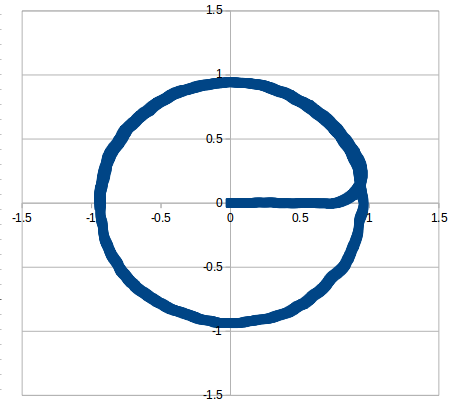
\includegraphics[width=\textwidth]{A3_Tracking_0001.png}
        \caption{\(\Sigma^2 = [0.001\ 0.001\ 0.001]\)}
    \end{subfigure}
    \begin{subfigure}{0.45\textwidth}
        \centering
        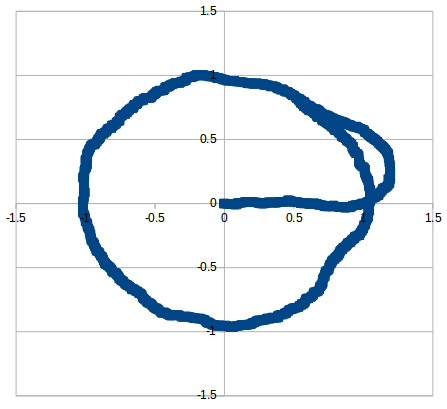
\includegraphics[width=\textwidth]{A3_Tracking_0100.png}
        \caption{\(\Sigma^2 = [0.1\ 0.1\ 0.1]\)}
    \end{subfigure}
    \caption{Trajectory Tracking}
\end{figure}
\end{frame}

\subsection{RMSE}
\begin{frame}{Root Mean Square Error}
\begin{itemize}
    \item Due to lack of individual state variable data in the above plot, the RMSE has been calculated as the distance from the required trajectory, which is the unit-radius circle about the origin.
    \item The RMSE has been calculated as follows: \[RMSE = \sqrt{\frac{\sum_{i=1}^N\left((x_i^2+y_i^2)-1\right)^2}{N}}\]
    \item The hence calculated RMSE for variance \(\Sigma^2 = [0.10\ 0.10\ 0.10]\) turns out to be around 0.15
\end{itemize}
\end{frame}

\section{A4}

\begin{frame}{Assignment 4}
  \centering
  \textbf{Assignment 04:\\Kalman Filter}
\end{frame}

\subsection{Progress}
\begin{frame}{Progress}
\begin{itemize}
    \item The scripts for this assignment has been completed.
    \item There exist certain bugs with respect to the matrix multiplication and inversion for the development of the Kalman filter. As a result, the workspace is not completely functional.
\end{itemize}
\end{frame}

\end{document}